\lecture{13. Review}{13}

%------------------------------------------------------------------------------
\section{Introduction}

%--------------------------------------
\begin{frame}{God wants a relationship with people}
\framesubtitle{Jeremiah 31:31-34}
\keyverse	
\note{09:30}
\end{frame}

%--------------------------------------
\begin{frame}
\frametitle{What makes Jer. 31:31-34 special?}
\framesubtitle{It describes what will change from the old covenant to the new.}
\begin{columns}
\begin{column}{0.4\textwidth}
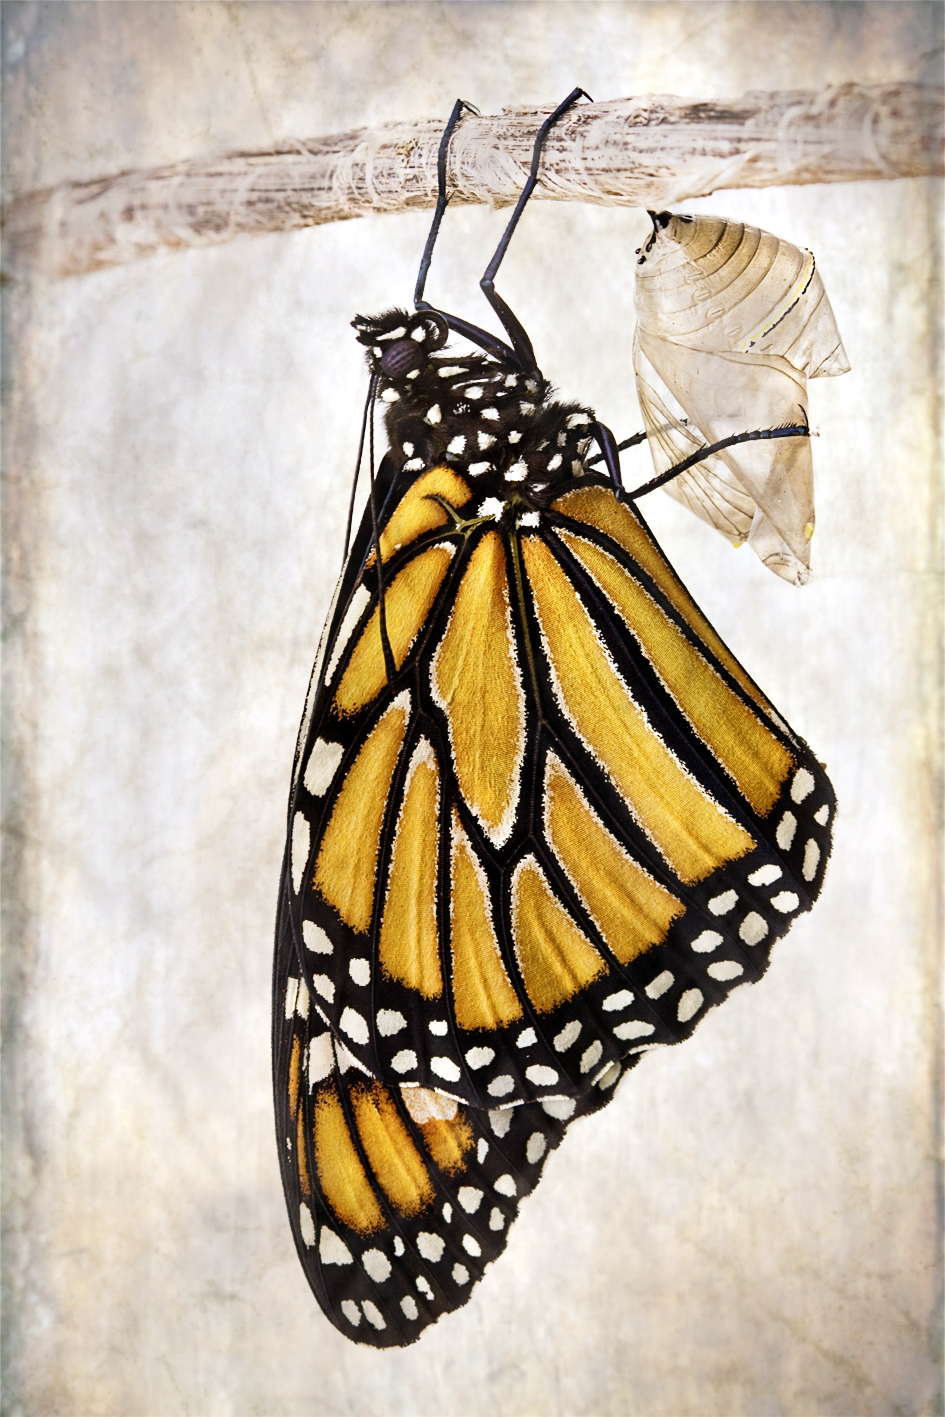
\includegraphics[width=\columnwidth]{figures/metamorphosis.jpg}
\end{column}
\begin{column}{0.6\textwidth}
\begin{itemize}
\item It is the only Old Testament verse with the term `new covenant'.
\item It contrasts old covenant faults with new covenant benefits.\\{\footnotesize (Heb. 8:1-13)}
\item It has the repeated Bible phrase, ``I will be their God and they shall be my people.'', which emphasizes relationship.\\{\footnotesize (Ex. 6:1-9, Lev. 22:31-33, etc.)}
\item It connects forgiveness of sins to our relationship with God.\\ {\footnotesize(John 3:16)}
\end{itemize}
\end{column}
\end{columns}
\end{frame}

\note{09:32}

%------------------------------------------------------------------------------
\section{The Big Picture}

%--------------------------------------
\begin{frame}
\frametitle{Class Objectives}
	\begin{columns}
	\begin{column}{0.4\textwidth}
		
\includegraphics[width=\columnwidth]{figures/objectives.jpg}
	\end{column}
	\begin{column}{0.6\textwidth}
		\begin{itemize}
		\item Know the big picture of the Bible:\\\emph{God wants a relationship with a holy people who voluntarily choose Him}
		\item Understand how the relationship between God and His people grew from the Old Covenant to the New Covenant.
		\item Develop a relationship perspective in your own walk with God.
		\end{itemize}
	\end{column}
	\end{columns}
	
	\note{09:34}
\end{frame}

%--------------------------------------
\begin{frame}
\frametitle{`I will be their God' through the Bible}
\begin{columns}[T]
	\begin{column}{0.45\textwidth}
		`I will be their God'\\{\footnotesize Gen. 17:8, Jer. 24:7, Jer. 31:33\\Jer. 32:36, Jer. 32:38, Ez. 11:20\\Ez. 37:15, Ez. 37:23, Ez. 37:27\\Zech. 8:8, 2 Cor. 6:16, Heb. 8:10}\\~\\
		`I will be your God'\\{\footnotesize Ex. 6:7, Jer. 7:23, Jer. 11:4\\Jer. 30:2, Ez. 36:28}\\~\\
	\end{column}
	\begin{column}{0.55\textwidth}
			`the Lord your God'\\ 
			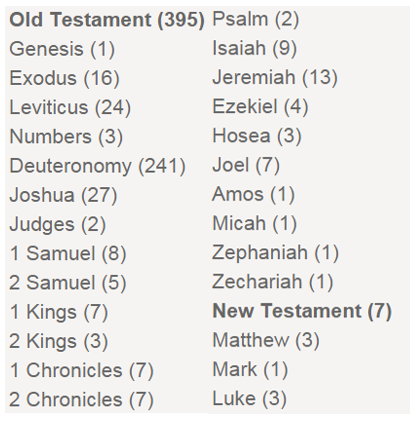
\includegraphics[width=1\columnwidth]{figures/theLordYourGodTwoColumn.png}
	\end{column}
\end{columns}

\note{09:37}
\note[item]{Last week, `your God', given to the Israelites as part of the Law of Moses (Ex. 6:1-9, Lev. 22:31-33).}
\note[item]{Clearly God thinks it's important that we view Him as the only God.}
\note[item]{It's not just that His people accept Him as the `true' God.  But as `their' God}
\end{frame}

%--------------------------------------
\begin{frame}
\frametitle{They shall be my people}
\framesubtitle{Matt 22:1-14}
\begin{center}

\includegraphics[height=0.7\textheight]{figures/different.jpg}\\
The people of God have to embrace being different.\\
You volunteered for this.
\end{center}

\note{09:37}
\note[item]{God's people will be special because He chose them.}
\note[item]{But, also because they chose Him.}
\note[item]{And, we're not different because we're somehow innately better than the world.}
\note[item]{On the contrary, the people who are called in the parable were the low people in society not the elites.}
\end{frame}

%--------------------------------------
\section{The Old Covenant}

%--------------------------------------
\begin{frame}
\frametitle{The covenant I made with their fathers}
\framesubtitle{Gal. 3:19-26}
\begin{columns}[c]
\begin{column}{0.4\textwidth}
	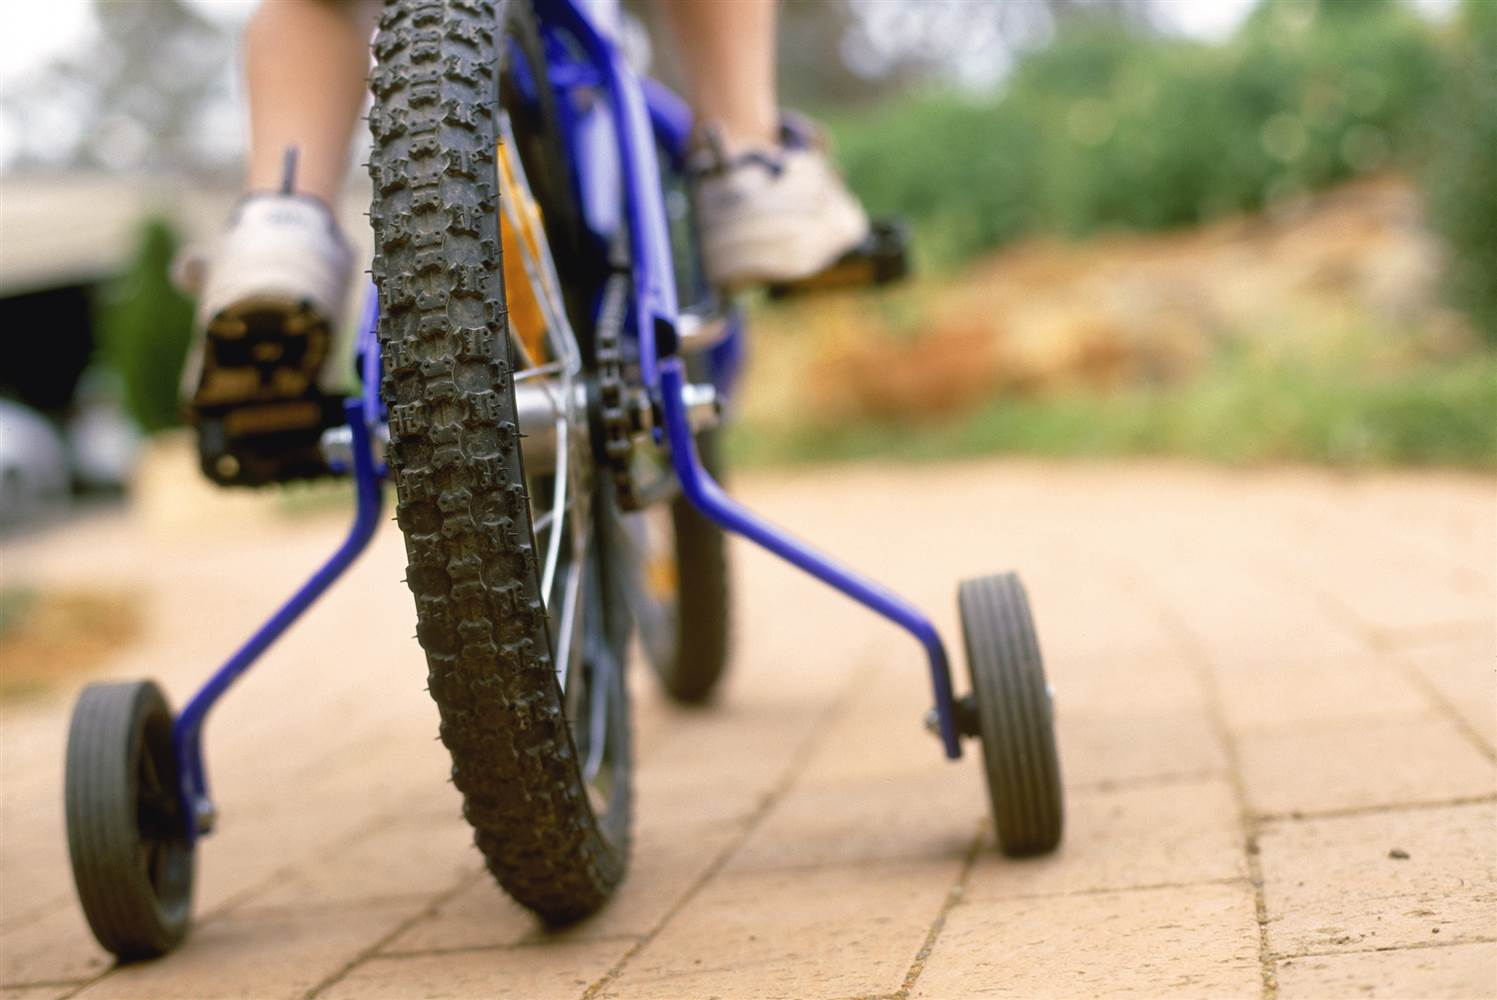
\includegraphics[width=\columnwidth]{figures/trainingWheels.jpg}
\end{column}
\begin{column}{0.6\textwidth}
	\emph{`added because of transgressions'}\\People tend to fall off the path\\~\\
	\emph{`a mediator is not for just one person, but God is one'}\\ Because Moses gave the Law to the Israelites, they didn't have a first hand relationship with God.\\~\\
	\emph{`was our guardian until Christ'}\\The Old Law constrained people to holy living when they didn't know much about the `plan'.
\end{column}
\end{columns}

\note{09:40}
\note[item]{The Message: The purpose of the law was to keep a sinful people in the way of salvation until Christ (the descendant) came, inheriting the promises and distributing them to us. Obviously this law was not a firsthand encounter with God. It was arranged by angelic messengers through a middleman, Moses. But if there is a middleman as there was at Sinai, then the people are not dealing directly with God, are they? But the original promise is the direct blessing of God, received by faith.}
\note[item]{The Old Covenant was a `guardian' to let people know what holy living looked like, until Jesus came}
\note[item]{But there were problems that came in how people used the Old Law\ldots}
\end{frame}

%--------------------------------------
\begin{frame}{I was a husband to them}
You can't make someone love you, but you can try and persuade
\begin{columns}[c]
\begin{column}{0.5\textwidth}
	
\includegraphics[width=\columnwidth]{figures/rose.jpg}
\end{column}
\begin{column}{0.5\textwidth}
  We all do this in marriage
	\begin{itemize}
    \item Things you give\ldots
		\begin{itemize}
			\item Communication
			\item Kindness
			\item Work around the house
      \item Take care of the kids
			\item Do your job(s)
			\item etc.
		\end{itemize}
    \item Responses you want\ldots
		\begin{itemize}
      \item Appreciation
      \item Kindness
      \item Closeness
			\item etc.
		\end{itemize}
	\end{itemize}
\end{column}
\end{columns}

\note{09:43}
\note[item]{Just as Jesus sacrificed Himself for us when we He wasn't loved in return, we should also give unselfishly to our spouse.}
\note[item]{Just like Jesus, though, we can hope that by our loving deeds, love will be returned.}
\note[item]{We do the same thing in marriage.}
\note[item]{God uses his acts of love to try and motivate us to love Him back, to live righteously, and to endure in our faith.}
\end{frame}

%--------------------------------------
\begin{frame}{My covenant they broke}
	\begin{itemize}
		\item Israel rejected God's love under the Old Covenant by \ldots
		\begin{itemize}
			\item not trusting God to take care of them to the promised land
			\item Worshiping idols while in the promised land
			\item Trying to rely only on works, but lacking faith
		\end{itemize}
		\item So they suffered the consequences \ldots
		\begin{itemize}
			\item The Exodus generation died in the wilderness
			\item Their descendants lost the promised land
			\item He was their only hope for salvation
		\end{itemize}
		\item Don't fall into their example \ldots
		\begin{itemize}
			\item Change when you face consequences.
			\item Pursue righteousness with faith.
			\item Trust that God will take care of you.
		\end{itemize}
	\end{itemize}
		
\note{09:46}
\end{frame}

\section{The New Covenant}

%--------------------------------------
\begin{frame}{The New Covenant vs. the Old}
\framesubtitle{Jer. 31:31-34}

\begin{description}[from the least to the greatest]
\item[I will put my law within them] genuine obedience
\item[I will write it on their hearts] inward commitment
\item[I will be their God] a new focus
\item[they shall be my people] it's no longer physical Israel
\item[\ldots they shall all know me] faith not genealogy
\item[from the least to the greatest] there's no distinctions
\item[I will forgive their iniquities] more than overlooking sins
\end{description}

\note{09:50}
\note[item]{write it on hearts -- not tablets.  Israelites should have done this (law `when you rise up and lay down').  Christians will get it right.}
\note[item]{God's covenant will become part of who we are}
\note[item]{Again, a separation existed in the Old Covenant.}
\note[item]{The separation was partly institutional, but mostly it was that people didn't internalize God's law.}
\end{frame}

%--------------------------------------
\begin{frame}{We've been brought near to God}
\framesubtitle{Eph 2}

\begin{columns}[c]
\begin{column}{0.4\textwidth}
	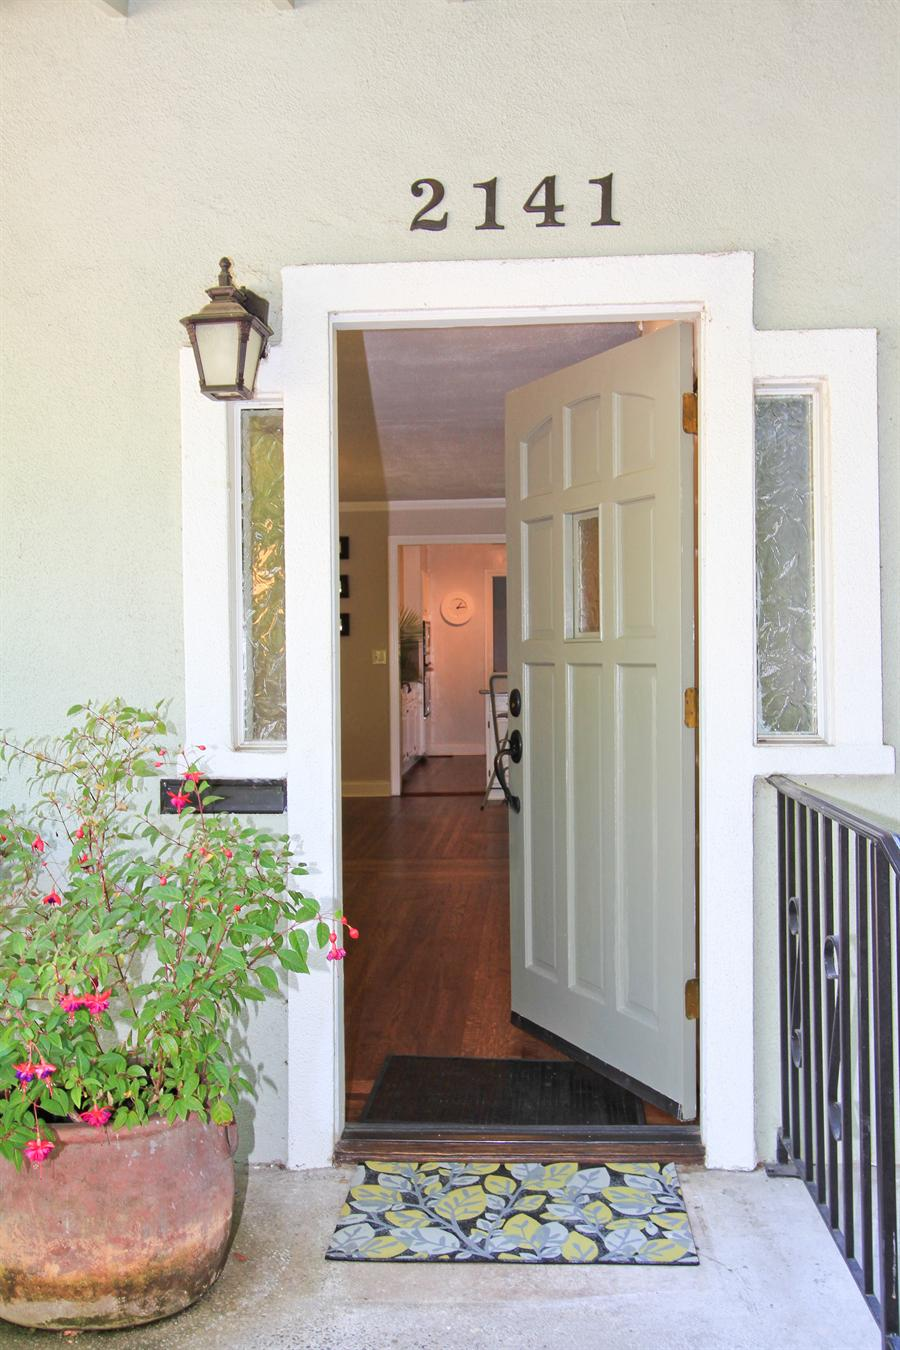
\includegraphics[width=\columnwidth]{figures/openDoor.jpg}
\end{column}
\begin{column}{0.6\textwidth}
	\begin{itemize}
		\item A seat in the heavens (6)
		\item Access to the Father (18)
		\item A member of God's household (19)
	\end{itemize}
\end{column}
\end{columns}

\note{9:58}
\end{frame}

%------------------------------------------------------------------------------
\section{Review}

\begin{frame}{Developing a New Covenant relationship with God}
	\begin{itemize}
		\item What passages from this class have had the greatest impact on you?  Why?
		\item Explain why developing an actual relationship with God is important.
		\item How will you continue to grow your relationship with God?
	\end{itemize}
	
\note{10:00}
\end{frame}
